\documentclass[10pt]{beamer}

% Aparência da apresentação (Tema moderno e limpo)
\usetheme{Madrid}
\usecolortheme{whale}

% Pacotes básicos
\usepackage[utf8]{inputenc}
\usepackage[portuguese]{babel}
\usepackage{graphicx}
\usepackage{booktabs}
\usepackage{amsmath}
\usepackage{amssymb}
\usepackage{listings}
\usepackage{xcolor}

% Configurações para exibição de códigos de programação
\lstset{
    language=Python,
    basicstyle=\ttfamily\tiny,
    keywordstyle=\color{blue},
    stringstyle=\color{red},
    commentstyle=\color{green!60!black},
    breaklines=true,
    showstringspaces=false
}

% Metadados da Apresentação
\title[Bootstrap e Testes A/B]{Bootstrap e Testes A/B}
\subtitle{Análise e Desenvolvimento de Sistemas}
\author[IFCE]{Prof. Reginaldo Fernandes\texorpdfstring{\\ \small{Adaptação Didática}}{ (IFCE)}}
\institute[IFCE Tauá]{Instituto Federal do Ceará -- Campus Tauá \\ Curso de Tecnologia em Análise e Desenvolvimento de Sistemas}
\date{\today}

\begin{document}

\begin{frame}
    \titlepage
\end{frame}

\begin{frame}{Sumário da Aula}
    \tableofcontents
\end{frame}

% Importando as seções da aula (Modularizado)
\section{Introdução e Problema da Inferência}

\begin{frame}{Como Conhecer a População?}
    \begin{block}{O Problema da Inferência}
        \begin{itemize}
            \item Temos acesso apenas a uma \textbf{amostra} de tamanho $N$.
            \item Nosso objetivo é descrever ou estimar propriedades da \textbf{população} (como a média $\mu$).
            \item Não temos orçamento ou meios para auditar a população completa.
        \end{itemize}
    \end{block}
    
    \begin{alertblock}{As Duas Abordagens Principais}
        \begin{enumerate}
            \item \textbf{Abordagem Clássica:} Utiliza fórmulas matemáticas baseadas em suposições rígidas de distribuição (ex: Teorema Central do Limite).
            \item \textbf{Abordagem Computacional:} Utiliza simulação e reamostragem a partir dos próprios dados observados (Bootstrap).
        \end{enumerate}
    \end{alertblock}
\end{frame}

\begin{frame}{O que é um Teste A/B?}
    \begin{block}{Definição Básica}
        Um experimento controlado para comparar duas versões de uma variável (A e B) com o objetivo de determinar qual delas é mais eficaz.
    \end{block}
    
    \begin{columns}
        \begin{column}{0.5\textwidth}
            \textbf{Grupo A (Controle)}
            \begin{itemize}
                \item Versão clássica do sistema.
                \item Experiência do usuário padrão.
                \item Medicamento placebo (em saúde).
            \end{itemize}
        \end{column}
        \begin{column}{0.5\textwidth}
            \textbf{Grupo B (Tratamento)}
            \begin{itemize}
                \item Nova funcionalidade ou design.
                \item Novo layout de checkout rápido.
                \item Novo princípio ativo.
            \end{itemize}
        \end{column}
    \end{columns}
    
    \vspace{0.4cm}
    \centering
    \textit{Queremos provar que a diferença observada entre os grupos é real, e não mera flutuação aleatória!}
\end{frame}

\begin{frame}{Exemplo Matemático: Estimativa de Parâmetros}
    \begin{block}{Problema de Negócio}
        Imagine que medimos o tempo de carregamento de uma página em 5 visitas (em segundos):
        $$X = \{1.5, 2.3, 1.8, 3.0, 2.4\}$$
        A estimativa pontual da média populacional $\mu$ é a média amostral $\bar{X}$:
        $$\bar{X} = \frac{1.5 + 2.3 + 1.8 + 3.0 + 2.4}{5} = \frac{11.0}{5} = 2.2\text{ s}$$
    \end{block}
    \begin{block}{Questão Fundamental}
        Essa estimativa pontual ($2.2\text{ s}$) é representativa? Se coletarmos outra amostra de 5 visitas, qual será a variação da média?
    \end{block}
\end{frame}

\begin{frame}[fragile]{Demonstração em Python: Média Amostral e Variabilidade}
    \begin{lstlisting}[language=Python]
import numpy as np

# Amostra de tempos de carregamento (em segundos)
X = np.array([1.5, 2.3, 1.8, 3.0, 2.4])

# Estimativa pontual da media
media_amostral = np.mean(X)
print(f"Media amostral: {media_amostral:.2f} s")
# Saida: Media amostral: 2.20 s

# Simulando a variabilidade amostral (se a populacao fosse conhecida)
np.random.seed(42)
populacao = np.random.normal(loc=2.2, scale=0.5, size=10000)
novas_medias = [np.random.choice(populacao, size=5).mean() for _ in range(1000)]
print(f"Desvio padrao das medias (erro padrao): {np.std(novas_medias):.3f}")
    \end{lstlisting}
\end{frame}


\section{O Método Clássico e o Teorema Central do Limite}

\begin{frame}{O Teorema Central do Limite (TCL)}
    \begin{block}{Definição}
        Independentemente da distribuição da população original, a distribuição da média amostral $\bar{X}$ se aproxima de uma distribuição normal à medida que o tamanho da amostra $N$ cresce.
    \end{block}
    
    \begin{block}{Intervalo de Confiança (IC) Clássico}
        O intervalo de 95\% de confiança para a média é dado por:
        $$IC = \bar{X} \pm 1.96 \times \frac{s}{\sqrt{N}}$$
        Onde $s$ é o desvio padrão amostral e $\frac{s}{\sqrt{N}}$ é o erro padrão (SE).
    \end{block}
\end{frame}

\begin{frame}{Limitações da Abordagem Clássica}
    \begin{alertblock}{Por que o TCL nem sempre é suficiente?}
        \begin{itemize}
            \item \textbf{Amostras pequenas:} Se a população for muito assimétrica e $N$ for pequeno, a aproximação normal falha.
            \item \textbf{Estatísticas complexas:} E se quisermos construir um intervalo de confiança para a \textbf{mediana}, \textbf{variância} ou uma razão entre variáveis? A matemática clássica torna-se extremamente complexa ou indisponível.
            \item \textbf{Outliers:} Presença de valores extremos distorce o desvio padrão e o erro padrão.
        \end{itemize}
    \end{alertblock}
    \centering
    \textbf{Solução em Ciência de Dados: Métodos Computacionais (Bootstrap)}
\end{frame}

\begin{frame}{Exemplo Matemático: IC via TCL}
    \begin{block}{Problema}
        Amostra de $N=36$ tempos de atendimento com média $\bar{X}=100\text{ s}$ e desvio padrão $s=15\text{ s}$. Queremos o IC de 95\% para a média populacional $\mu$.
    \end{block}
    \begin{block}{Cálculo Analítico (TCL)}
        \begin{itemize}
            \item \textbf{Erro padrão da média ($SE$):} $SE = \frac{s}{\sqrt{N}} = \frac{15}{\sqrt{36}} = 2.5\text{ s}$
            \item \textbf{Margem de erro (para $z = 1.96$):} $1.96 \times 2.5 = 4.9\text{ s}$
            \item \textbf{Intervalo de Confiança (95\%):} $IC = 100 \pm 4.9 = [95.1\text{ s}, 104.9\text{ s}]$
        \end{itemize}
    \end{block}
\end{frame}

\begin{frame}[fragile]{Demonstração em Python: IC Clássico}
    \begin{lstlisting}[language=Python]
import numpy as np
import scipy.stats as ss

# Dados amostrais simulados (N=36, media=100, std=15)
np.random.seed(42)
dados = np.random.normal(loc=100, scale=15, size=36)

# Calculos intermediarios
n = len(dados)
media = np.mean(dados)
desvio = np.std(dados, ddof=1) # Desvio padrao amostral
erro_padrao = desvio / np.sqrt(n)

# Encontrando o z critico para 95%
z_critico = ss.norm.ppf(0.975)

# Limites do intervalo
lim_inf = media - z_critico * erro_padrao
lim_sup = media + z_critico * erro_padrao
print(f"IC Classico: [{lim_inf:.2f}, {lim_sup:.2f}]")
# Saida aproximada: IC Classico: [94.59, 104.07]
    \end{lstlisting}
\end{frame}


\section{O Método Bootstrap}

\begin{frame}{O Princípio do Bootstrap}
    \begin{block}{Origem do Nome}
        Derivado da expressão \textit{"to pull oneself up by one's own bootstraps"} (erguer-se puxando as próprias botas). Remete a realizar uma tarefa impossível utilizando apenas os recursos disponíveis.
    \end{block}
    
    \begin{block}{Idéia Central}
        A amostra observada é a melhor representação disponível da população desconhecida. 
        Reamostrar \textbf{com reposição} dessa amostra imita o processo de retirar amostras da própria população original.
    \end{block}
\end{frame}

\begin{frame}{O Algoritmo do Bootstrap}
    \begin{enumerate}
        \item Considere uma amostra original $S$ de tamanho $N$.
        \item Crie uma nova amostra (reamostra bootstrap) sorteando $N$ elementos de $S$ \textbf{com reposição}.
        \item Calcule a estatística desejada (ex: média) para essa reamostra.
        \item Repita os passos 2 e 3 um número elevado de vezes (ex: $M = 5000$).
        \item Use a distribuição das estatísticas geradas para estimar variabilidade e limites de confiança.
    \end{enumerate}
\end{frame}

\begin{frame}{Exemplo Matemático: Bootstrap Manual}
    \begin{block}{Problema}
        Temos uma amostra inicial pequena $S = \{2, 4, 9\}$ com $N = 3$.
        A média observada é $\bar{X} = 5.0$.
        Vamos simular a amostragem com reposição para obter 4 reamostras bootstrap:
    \end{block}
    \begin{block}{Simulações de Reamostragem}
        \begin{itemize}
            \item \textbf{Reamostra 1:} $\{2, 2, 9\} \rightarrow \bar{X}^*_1 = \frac{13}{3} \approx 4.33$
            \item \textbf{Reamostra 2:} $\{4, 9, 9\} \rightarrow \bar{X}^*_2 = \frac{22}{3} \approx 7.33$
            \item \textbf{Reamostra 3:} $\{2, 4, 4\} \rightarrow \bar{X}^*_3 = \frac{10}{3} \approx 3.33$
            \item \textbf{Reamostra 4:} $\{9, 2, 9\} \rightarrow \bar{X}^*_4 = \frac{20}{3} \approx 6.67$
        \end{itemize}
        A distribuição das médias bootstrap obtida é $\{3.33, 4.33, 6.67, 7.33\}$.
        Em escala real, faríamos isso 5000 vezes para obter percentis estáveis.
    \end{block}
\end{frame}

\begin{frame}[fragile]{Demonstração em Python: Bootstrap Manual}
    \begin{lstlisting}[language=Python]
import numpy as np

# Amostra original
S = np.array([2, 4, 9])
n = len(S)

# Gerando reamostras com reposicao
np.random.seed(42)
m = 4 # Apenas 4 reamostras para ilustrar
medias_bs = []

for i in range(m):
    reamostra = np.random.choice(S, size=n, replace=True)
    media_tmp = reamostra.mean()
    medias_bs.append(media_tmp)
    print(f"Reamostra {i+1}: {reamostra} -> Media: {media_tmp:.2f}")

# Calculo de percentil com 10000 simulacoes para IC de 95%
todas_medias = [np.random.choice(S, size=n, replace=True).mean() for _ in range(10000)]
ic_bs = np.percentile(todas_medias, [2.5, 97.5])
print(f"IC Bootstrap (95%): [{ic_bs[0]:.2f}, {ic_bs[1]:.2f}]")
    \end{lstlisting}
\end{frame}

\begin{frame}[fragile]{Implementação da Média via Bootstrap}
    \begin{lstlisting}[language=Python]
def bootstrap_mean(df, column, n=5000, size=None):
    if size is None:
        size = len(df)
    values = np.zeros(n)
    data_array = df[column].to_numpy()
    for i in range(n):
        # Amostragem com reposicao (replace=True)
        sample = np.random.choice(data_array, size=size, replace=True)
        values[i] = sample.mean()
    return values
    \end{lstlisting}
    
    \begin{block}{Intervalo de Confiança Bootstrap}
        Calculado a partir dos percentis empíricos da distribuição obtida (ex: 2.5\% e 97.5\%):
        \lstinline[language=Python]!np.percentile(values, [2.5, 97.5])!
    \end{block}
\end{frame}

\begin{frame}{Demonstração de Convergência}
    \begin{columns}
        \begin{column}{0.45\textwidth}
            \begin{itemize}
                \item À medida que aumentamos o número de amostras bootstrap ($M$), a estimativa empírica se estabiliza.
                \item Em distribuições padrão, o IC Bootstrap converge para o IC Clássico do TCL.
            \end{itemize}
        \end{column}
        \begin{column}{0.55\textwidth}
            \centering
            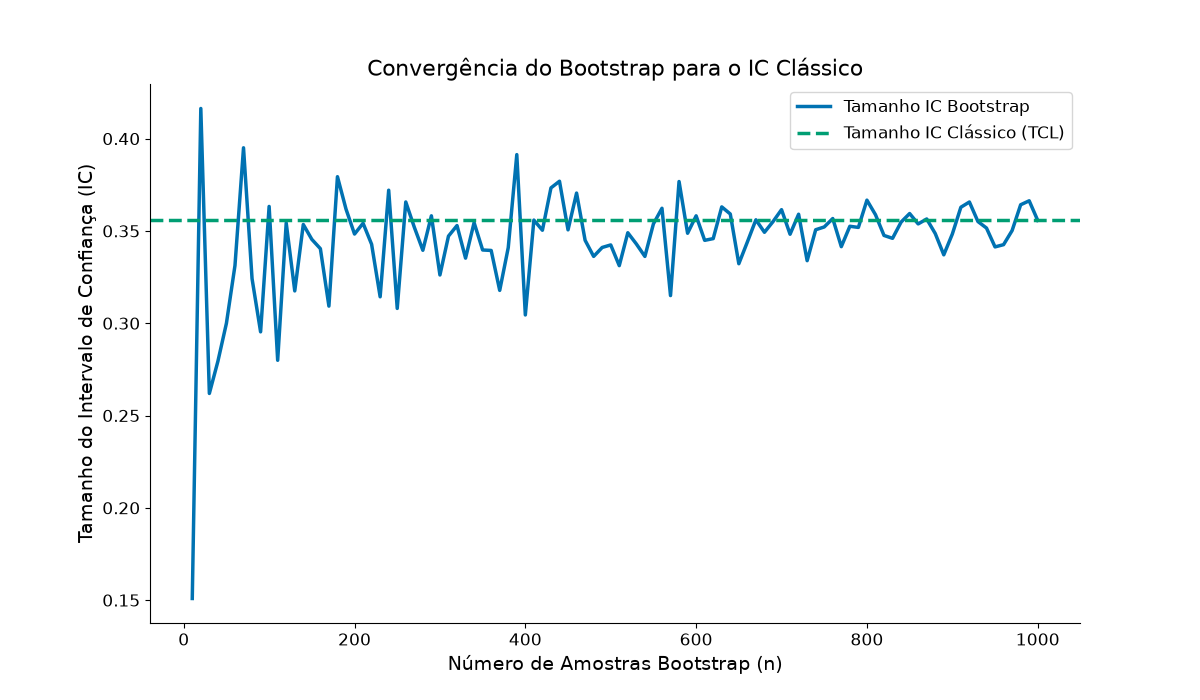
\includegraphics[width=\textwidth]{01_convergencia_sintetica.png}
        \end{column}
    \end{columns}
\end{frame}

\section{Testes A/B Computacionais}

\begin{frame}{Comparando Dois Grupos Independentes}
    \begin{block}{Duas Abordagens Didáticas}
        \begin{enumerate}
            \item \textbf{Sobreposição de ICs Individuais:} Calcular o IC para cada grupo separadamente e checar se eles se sobrepõem. (Abordagem conservadora).
            \item \textbf{IC da Diferença das Médias (Padrão):} Estimar diretamente a distribuição bootstrap de $\bar{X}_1 - \bar{X}_2$. Se o intervalo correspondente contiver o valor zero, dizemos que não há diferença significativa entre as médias.
        \end{enumerate}
    \end{block}
\end{frame}

\begin{frame}{Exemplo Matemático: Diferença de Médias via Bootstrap}
    \begin{block}{Problema}
        Grupos: $X_A = \{10, 15, 20\} \rightarrow \bar{X}_A = 15.0$ e $X_B = \{12, 18, 24\} \rightarrow \bar{X}_B = 18.0$.
        Diferença observada: $+3.0$. Vamos reamostrar com reposição:
    \end{block}
    \begin{block}{Simulações de Reamostragem}
        \begin{itemize}
            \item \textbf{Passo 1:} Reamostras $B^*_1 = \{18, 24, 24\}$ (méd. $22.0$) e $A^*_1 = \{15, 15, 20\}$ (méd. $16.67$). Diferença: $22.0 - 16.67 = 5.33$.
            \item \textbf{Passo 2:} Reamostras $B^*_2 = \{12, 12, 18\}$ (méd. $14.0$) e $A^*_2 = \{10, 20, 20\}$ (méd. $16.67$). Diferença: $14.0 - 16.67 = -2.67$.
        \end{itemize}
        Repetindo 5000 vezes, analisamos se a diferença é significativamente maior que zero.
    \end{block}
\end{frame}

\begin{frame}[fragile]{Demonstração em Python: Teste A/B Simples}
    \begin{lstlisting}[language=Python]
import numpy as np

# Grupos originais
grupo_A = np.array([10, 15, 20])
grupo_B = np.array([12, 18, 24])

# Simulando a diferenca das medias
np.random.seed(42)
diferencas_bs = []

for _ in range(5000):
    resample_A = np.random.choice(grupo_A, size=len(grupo_A), replace=True)
    resample_B = np.random.choice(grupo_B, size=len(grupo_B), replace=True)
    diferencas_bs.append(resample_B.mean() - resample_A.mean())

# Intervalo de Confianca de 95% para a diferenca
ic_diferenca = np.percentile(diferencas_bs, [2.5, 97.5])
print(f"IC da diferenca (95%): [{ic_diferenca[0]:.2f}, {ic_diferenca[1]:.2f}]")
# Saida: IC da diferenca (95%): [-3.67, 9.67]. Contem zero, nao e significativa!
    \end{lstlisting}
\end{frame}


\begin{frame}[fragile]{Caso de Estudo 1: Saúde Pública}
    \begin{block}{Peso de Bebês e Tabagismo Materno}
        \begin{itemize}
            \item \textbf{Dados:} Amostra de recém-nascidos (\texttt{baby.csv}).
            \item \textbf{Grupo Controle:} Mães não fumantes.
            \item \textbf{Grupo Tratamento:} Mães fumantes.
        \end{itemize}
    \end{block}
    
    \begin{lstlisting}[language=Python]
# Codigo para calcular diferenca de medias via bootstrap
def bootstrap_diff(df1, df2, column, n=5000):
    data1 = df1[column].to_numpy()
    data2 = df2[column].to_numpy()
    diff_values = np.zeros(n)
    for i in range(n):
        s1 = np.random.choice(data1, size=len(df1), replace=True)
        s2 = np.random.choice(data2, size=len(df2), replace=True)
        diff_values[i] = s1.mean() - s2.mean()
    return diff_values
    \end{lstlisting}
\end{frame}

\begin{frame}[fragile]{Código Completo: Carga, Preparação e Bootstrap}
    \begin{lstlisting}[language=Python]
import pandas as pd
import numpy as np

# 1. Carregar dados da URL
url = 'https://media.githubusercontent.com/media/icd-ufmg/material/master/aulas/10-AB/baby.csv'
df = pd.read_csv(url)

# 2. Conversao de unidades (oncas para kg)
df['Birth Weight'] = 0.0283495 * df['Birth Weight']

# 3. Separar em grupos: Controle vs Tratamento
smokers = df[df['Maternal Smoker'] == True]
no_smokers = df[df['Maternal Smoker'] == False]

# 4. Rodar o bootstrap para a diferenca das medias
np.random.seed(42)
diferencas = bootstrap_diff(smokers, no_smokers, 'Birth Weight', n=5000)

# 5. Calcular o IC de 95 por cento para a diferenca
ic_95 = np.percentile(diferencas, [2.5, 97.5])
print(f"IC 95%: [{ic_95[0]:.3f} kg, {ic_95[1]:.3f} kg]")
    \end{lstlisting}
\end{frame}

\begin{frame}{Resultados: Peso de Bebês}
    \begin{itemize}
        \item \textbf{Média não fumantes:} $3.489\text{ kg}$
        \item \textbf{Média fumantes:} $3.227\text{ kg}$
        \item \textbf{Diferença observada:} $-0.263\text{ kg}$
        \item \textbf{IC de 95\% para a diferença (Bootstrap):} $[-0.323, -0.202]\text{ kg}$
    \end{itemize}
    
    \begin{alertblock}{Conclusão Estatística}
        Como o intervalo $[-0.323, -0.202]\text{ kg}$ \textbf{não inclui o valor zero}, rejeitamos a hipótese de igualdade entre as médias. Há diferença estatística significativa.
    \end{alertblock}
\end{frame}

\begin{frame}{Visualização: Distribuições de Médias Bootstrap}
    \centering
    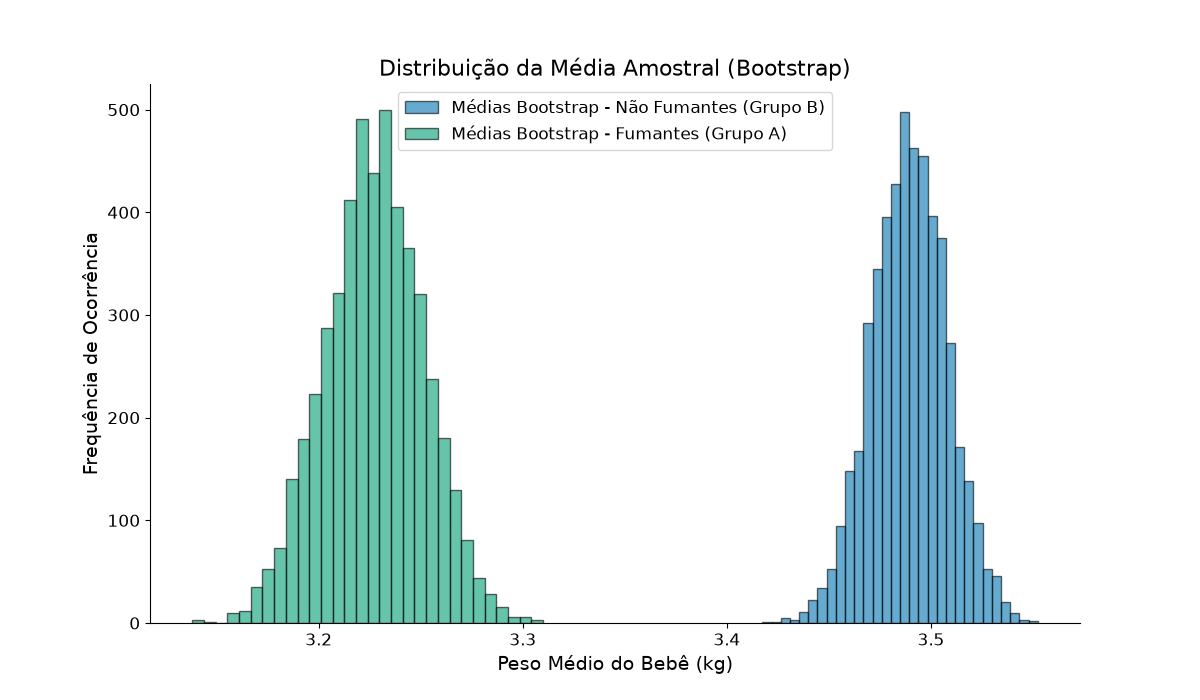
\includegraphics[width=0.85\textwidth]{02_medias_bootstrap.png}
\end{frame}

\begin{frame}{Explicação: Distribuições das Médias Bootstrap}
    \begin{block}{Interpretação das Médias Individuais}
        \begin{itemize}
            \item \textbf{Mães Não Fumantes (azul):} A distribuição das médias amostrais $\bar{X}$ (média amostral) está centrada em $3.49\text{ kg}$, variando no $IC$ (Intervalo de Confiança) de $[3.45, 3.52]\text{ kg}$.
            \item \textbf{Mães Fumantes (laranja):} A distribuição está centrada em $3.23\text{ kg}$, variando no $IC$ (Intervalo de Confiança) de $[3.18, 3.27]\text{ kg}$.
            \item \textbf{Ausência de Sobreposição:} Como os $IC$ (Intervalos de Confiança) dos dois grupos não se sobrepõem, há um indício inicial muito forte de que o peso médio populacional é diferente entre os grupos.
        \end{itemize}
    \end{block}
\end{frame}

\begin{frame}{Visualização: Diferença de Médias e ECDF}
    \centering
    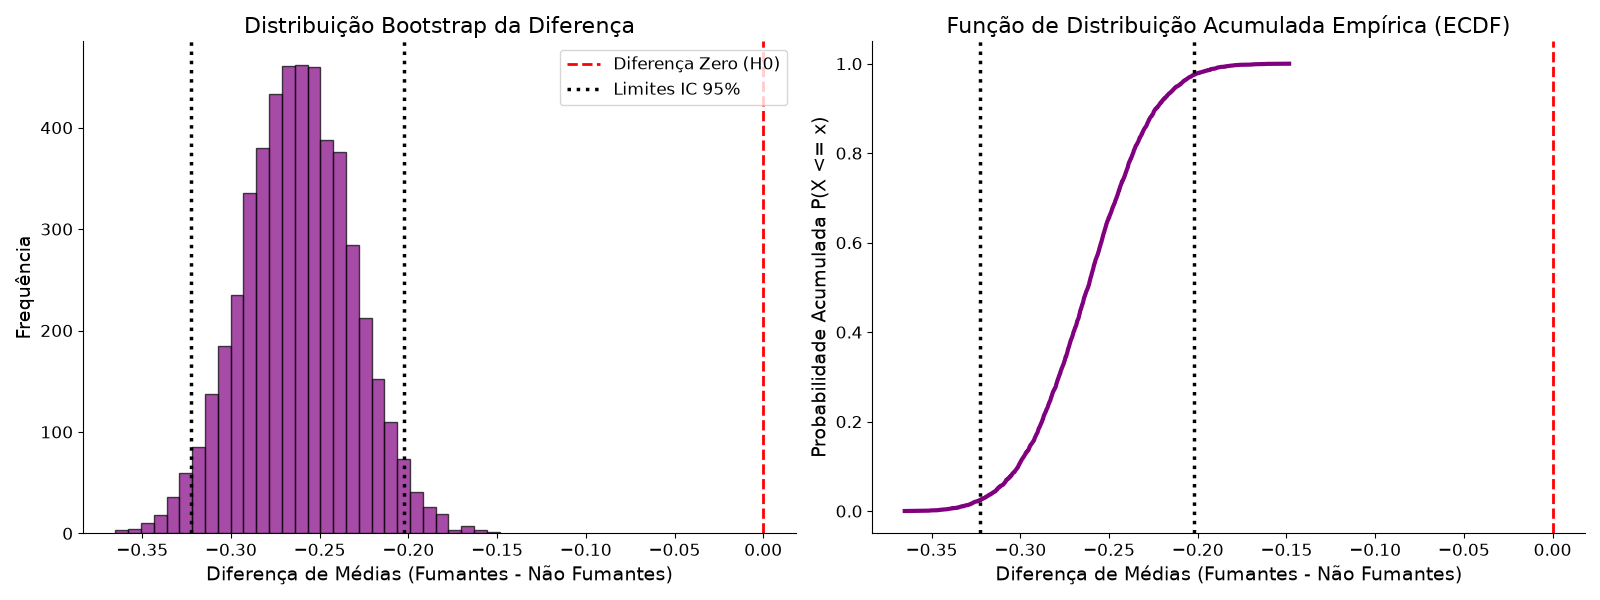
\includegraphics[width=0.9\textwidth]{03_diferenca_ecdf.png}
\end{frame}

\begin{frame}{Explicação: Efeito da Diferença e ECDF}
    \begin{block}{Análise da Diferença e da ECDF}
        \begin{itemize}
            \item \textbf{Distribuição da Diferença (Esquerda):} Mostra a distribuição de todas as $5.000$ diferenças simuladas $\bar{d}^* = \bar{X}^*_{\text{Fumantes}} - \bar{X}^*_{\text{Não Fumantes}}$. O $IC$ (Intervalo de Confiança) de 95\% da diferença é $[-0.323, -0.202]\text{ kg}$ (totalmente abaixo de zero).
            \item \textbf{Curva ECDF (Direita):} A $ECDF$ (Função de Distribuição Acumulada Empírica) chega ao topo ($1.0$ ou 100\% de probabilidade acumulada) bem antes do ponto zero no eixo horizontal.
            \item \textbf{Conclusão:} A probabilidade de a diferença ser maior ou igual a zero é nula ($P(\bar{d}^* \ge 0) = 0$), comprovando o efeito negativo do fumo.
        \end{itemize}
    \end{block}
\end{frame}

\begin{frame}{Caso de Estudo 2: UX e E-commerce}
    \begin{block}{Impacto de Checkout Expresso no Ticket Médio}
        \begin{itemize}
            \item \textbf{Layout A (Controle):} Checkout em múltiplos passos (250 vendas). Média: R\$44.75.
            \item \textbf{Layout B (Tratamento):} Novo Checkout Expresso (200 vendas). Média: R\$47.29.
        \end{itemize}
    \end{block}
    
    \begin{block}{Simulação Bootstrap do Ticket Médio}
        \begin{itemize}
            \item Diferença de médias observada (B - A): $+\text{R\$} 2.53$
            \item IC de 95\% da diferença: $[\text{R\$} 0.18, \text{R\$} 4.90]$
            \item \textbf{Conclusão:} Como o limite inferior de R\$0.18 está acima de zero, podemos afirmar que o novo layout gerou aumento de receita.
        \end{itemize}
    \end{block}
\end{frame}

\begin{frame}{Visualização: Dispersão do Ticket Médio}
    \centering
    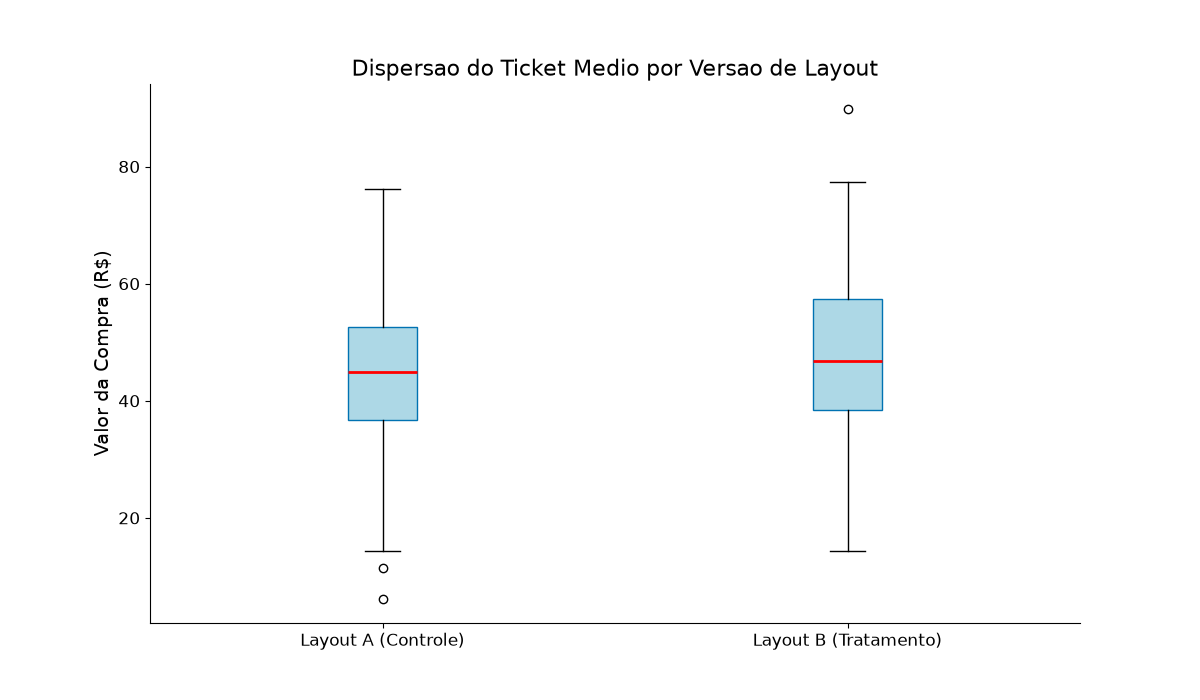
\includegraphics[width=0.85\textwidth]{05_boxplot_ecommerce.png}
\end{frame}

\begin{frame}{Explicação: Boxplot de Vendas}
    \begin{block}{Entendendo a Dispersão dos Dados}
        \begin{itemize}
            \item \textbf{O Boxplot:} O gráfico de caixa mostra a mediana (linha vermelha), a caixa central contendo o $IQR$ (Intervalo Interquartil - do 1º ao 3º quartil) e as caudas (limites mínimo e máximo).
            \item \textbf{Layout A (Controle):} Mediana ligeiramente abaixo de $45$, com a maioria dos tickets distribuídos de forma simétrica.
            \item \textbf{Layout B (Tratamento):} Mediana claramente acima do Layout A. A caixa inteira e seus quartis estão deslocados para cima.
            \item \textbf{Interpretação:} Embora haja uma grande sobreposição das compras individuais (variabilidade natural), a tendência central do Layout B está visivelmente deslocada para valores mais altos. O Bootstrap nos ajudará a inferir se essa diferença de média é real.
        \end{itemize}
    \end{block}
\end{frame}

\begin{frame}{Visualização: Teste A/B E-commerce}
    \centering
    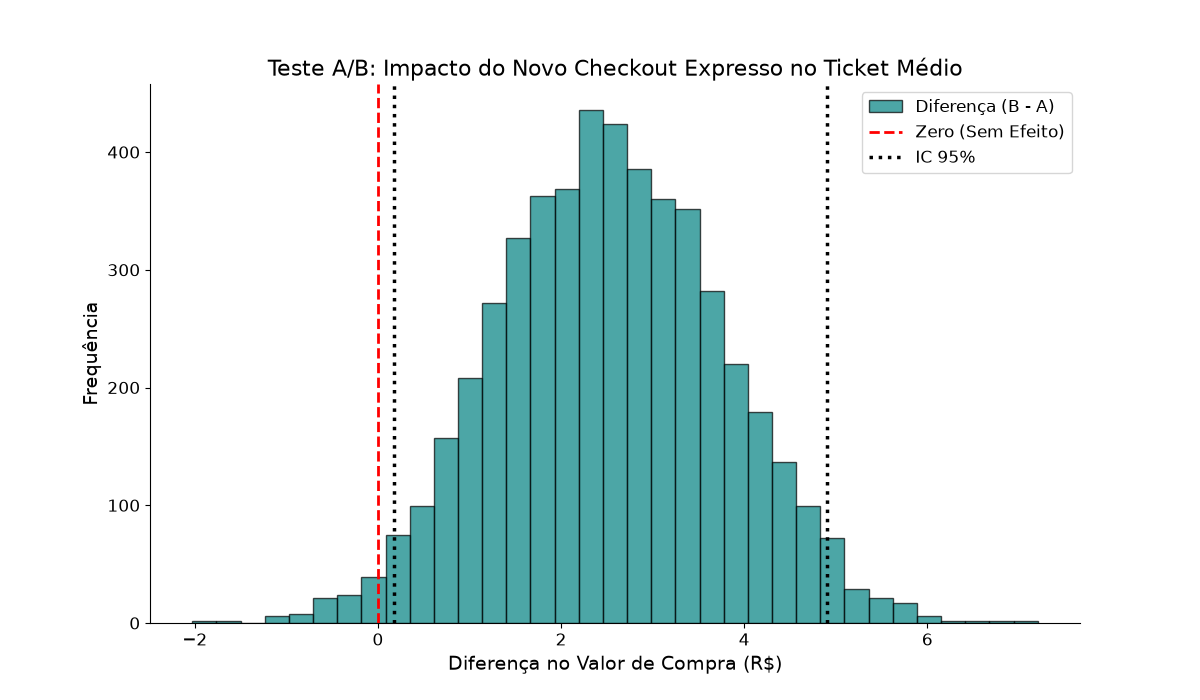
\includegraphics[width=0.85\textwidth]{04_ab_teste_ecommerce.png}
\end{frame}

\begin{frame}{Explicação: Teste A/B de Ticket Médio}
    \begin{block}{Interpretação de Negócio (Checkout Expresso)}
        \begin{itemize}
            \item \textbf{Efeito Estimado:} A diferença observada de ticket médio ($B - A$) é de $+\text{R\$} 2.53$.
            \item \textbf{Decisão Estatística:} O $IC$ (Intervalo de Confiança) de 95\% da diferença obtida via Bootstrap é $[\text{R\$} 0.18, \text{R\$} 4.90]$.
            \item \textbf{Ausência de Zero:} Como o limite inferior do $IC$ (Intervalo de Confiança) está estritamente acima de zero, o novo Layout B traz um ganho real e não puramente aleatório. Recomendamos implementar em produção.
        \end{itemize}
    \end{block}
\end{frame}


\section{Consolidação e Exercícios}

\begin{frame}{Resumo e Melhores Práticas}
    \begin{block}{Quando usar o Bootstrap?}
        \begin{itemize}
            \item Distribuições altamente distorcidas (Ex: renda, acessos a servidores).
            \item Amostras médias e pequenas onde as premissas clássicas falham.
            \item Ao estimar estatísticas não-lineares (mediana, variâncias, razões).
        \end{itemize}
    \end{block}
    
    \begin{alertblock}{Armadilhas em Testes A/B}
        \begin{itemize}
            \item \textbf{Peeking (Espiadinha):} Olhar os resultados do teste toda hora e parar assim que der significância infla falsos positivos.
            \item \textbf{Significância Estatística vs. Prática:} Ganho estatisticamente comprovado de 0,001\% pode não valer o custo de engenharia.
        \end{itemize}
    \end{alertblock}
\end{frame}

\begin{frame}{Exercícios Propostos}
    \begin{enumerate}
        \item \textbf{Modifique para a Mediana:} Altere a função \texttt{bootstrap\_mean} para calcular a mediana e compare os resultados de renda da base de dados fornecida.
        \item \textbf{Análise do Tamanho Amostral ($N$):} Varie o tamanho da amostra inicial no script de apoio e responda: Como o tamanho da amostra inicial impacta a largura final do Intervalo de Confiança Bootstrap?
        \item \textbf{Construção de Histograma:} Utilizando o script \texttt{aula10\_pratica.py}, execute o exemplo de e-commerce, salve a imagem gerada e plote os limites no gráfico.
    \end{enumerate}
\end{frame}


\end{document}
